\setcounter{chapter}{7}
\setcounter{section}{0}
\setcounter{figure}{0}
\setcounter{equation}{0}
\setcounter{table}{0}
\chapter*{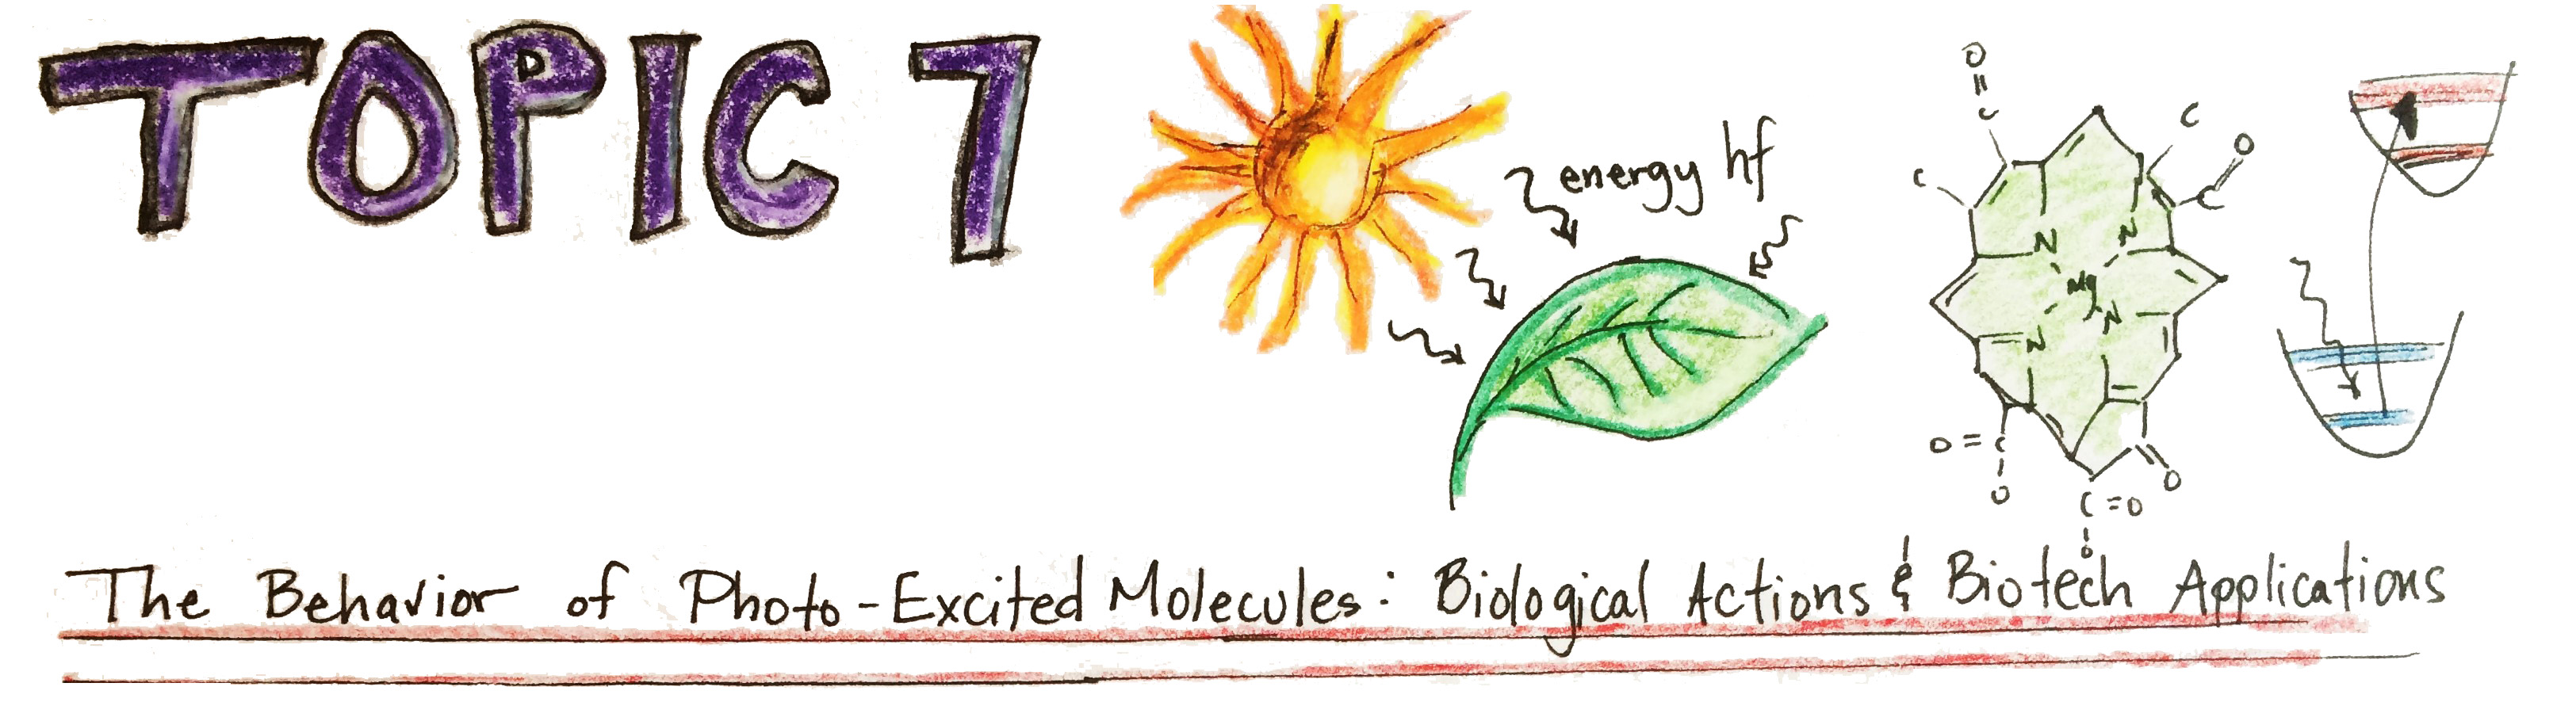
\includegraphics[width=\textwidth]{./figures/Topic7/Topic7.jpg}}
\addcontentsline{toc}{chapter}{Topic 7: The Behavior of Photo-Excited Molecules:
Biological Actions and Biotechnological Applications}

\section{Introduction}

Topic 6 gave us a foundation for understanding the process of light absorption in organic molecules.  We now know that when a photon strikes a molecule, one of its electrons can absorb the energy and be promoted to an excited state. What happens next? Does the molecule retain that energy indefinitely? Is it converted into other forms? Here we discuss the fundamental processes that ensue from light absorption, and their relevance to biology as well as important biotechnological applications. 

\section{Kasha's Rule}

 In 1953, Michael Kasha proposed that no matter how much light energy a molecule absorbs, it undergoes a rapid transition to the first excited state.  Since the transition occurs typically in less than one picosecond, we can assume that the molecule will always be effectively excited to the first excited state regardless of the energy carried by the photon. The process is sown in Fig.~\ref{Fig7-1}. Furthermore, the transition from higher excited states to the first excited state usually emits no light, and is thus categorized as a radiationless transition.
\begin{figure}[h]
	\centering
	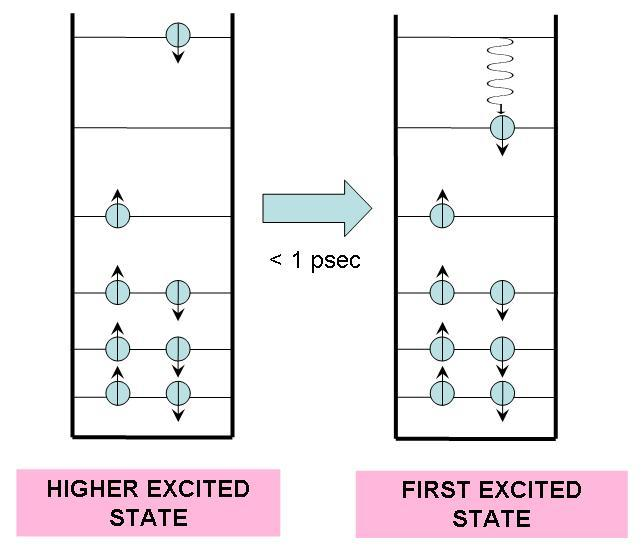
\includegraphics[width=4.0in]{./figures/Topic7/Fig7-1.jpg}
	\caption{If a molecule is excited to an energy level higher than the first excited state, it undergoes a radiationless transition to this state, releasing excess heat into its environment.}
	\label{Fig7-1}
\end{figure}
In a radiationless transition, the electronic energy difference is converted into vibrational energy.  This results in a higher internal temperature for the molecule, but it quickly (within 10 ps) returns to ambient temperature by releasing heat into the surrounding medium.

From the first excited state, the molecule can proceed in one of many ways.  In this chapter we will examine six possible outcomes for an excited molecule: radiationless transition to the ground state; fluorescence; intersystem crossing; phosphorescence; excitation transfer to another nearby molecule; and charge transfer to another nearby molecule.  We will also discuss several biological systems and technologies that take advantage of these photophysical phenomena.

\section{Radiationless Transition to the Ground State}

A radiationless transition to the ground state is essentially the same as a radiationless transition from higher excited states to the first excited state, described in section 7.2.  The only difference is that the molecule now transitions from the first excited state to the ground state.  No photons are emitted, and the excess energy is converted to heat, which is quickly released into the surrounding medium. 
\begin{figure}[h]
	\centering
	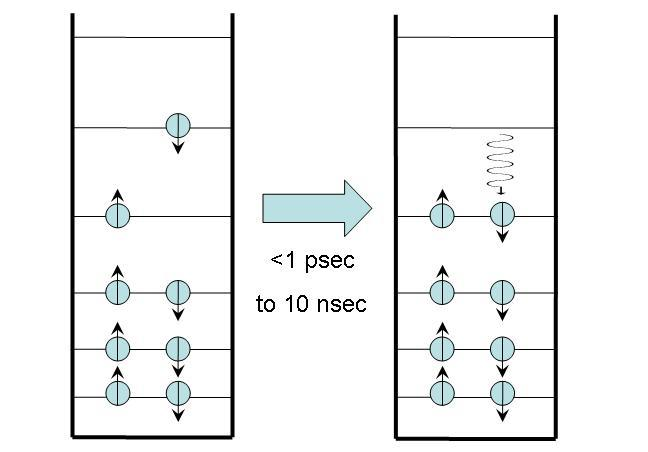
\includegraphics[width=4.0in]{./figures/Topic7/Fig7-2.jpg}
	\caption{Radiationless transfer to the ground state.}
	\label{Fig7-2}
\end{figure}
This process usually takes place on a nanosecond timescale, substantially longer than radiationless transitions from higher excited states.  Some molecules -- such as metalloporphyrins like hemes and cytochromes -- decay to the ground state very quickly, within a few picoseconds.  This fast decay is due to the presence of iron in the center of these molecules, which creates additional electronic states between the first excited state and the ground state that facilitate the decay.  Temperatures can reach 200$^{\circ}$C inside these molecules when the energy is converted to heat, but the heat is dissipated so quickly that the molecules suffer no damage.

\section{Fluorescence}

In fluorescence, as shown in Fig.~\ref{Fig7-2}, the molecule begins in an excited state with no net spin, as all the spins of the electrons cancel each other out.  Within nanoseconds, a photon is emitted and the molecule returns to ground state.  The net spin remains zero.  The energy lost by the electron inside the molecule is entirely converted into photon energy.
\begin{figure}[h]
	\centering
	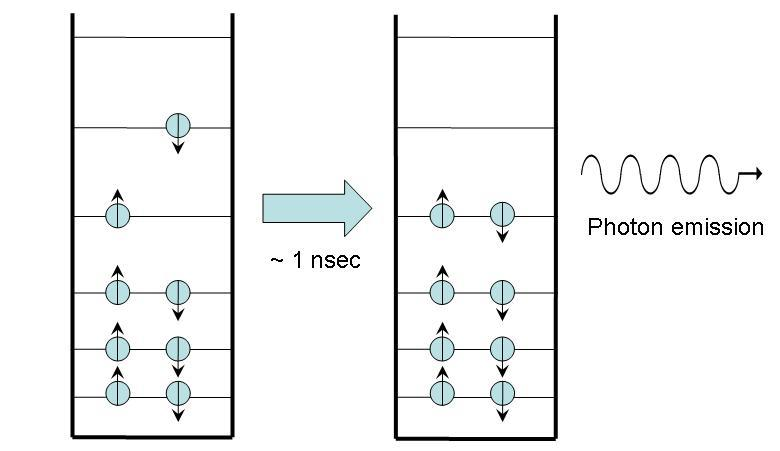
\includegraphics[width=4.0in]{./figures/Topic7/Fig7-3.jpg}
	\caption{Fluorescence. Note that the photon emitted has the same energy as the energy difference between the excited and ground states.}
	\label{Fig7-3}
\end{figure}
You are familiar with fluorescence if you have ever seen your clothes ``glow'' under a black light.  Most light-colored fabrics absorb some blue light, so they tend to naturally appear yellowish, even when clean.  To make them look whiter, we wash them with detergents that contain ``whiteners,'' small fluorescent molecules that adhere to fabric.  Illuminating detergent with ultraviolet light causes it to fluoresce bright blue.  The added blue light emanating from the detergent molecules causes the fabric to appear whiter.

When isolated from their natural environment, most biological molecules exhibit a significant amount of fluorescence.  For example, if you grind leaves from a green plant and suspend the particles in solution so that the pigment molecules are isolated from one another, the solution will fluoresce red-orange under ultraviolet light.  Not all biomolecules do this; however, exceptions include heme and the cytochromes, which undergo a radiationless transition before they have a chance to fluoresce.

In vivo, however, most biological molecules display modest fluorescence, particularly within the visible range.  Either the fluorescence does occur but is quickly reabsorbed by surrounding molecules, or the molecule transfers the energy or an electron to a nearby molecule.  An exception to the lack of in vivo fluorescence occurs in association with the rare genetic disease porphyria.  One form of the disease is caused by an enzyme that fails to catalyze the binding of iron to the porphyrin ring of heme.  The porphyrins build up over time in the teeth and bones, which, if irradiated with UV light display a reddish fluorescence.

\section{Intersystem Crossing}

In intersystem crossing, the molecule begins in an excited state with a net spin of 0 because all electron spins cancel one another. After a time, typically 10 nsec or longer, it ends in an excited state with a net spin of 1 (i.e. a spin angular momentum with a magnitude equal to $\hbar$ or $h/2\pi$.  This end state is called a triplet state because of a quantum mechanical effect that produces three possible states with different angular momentum orientations \footnote[3]{In general, quantum mechanical systems are allowed to change their angular momentum, but only in increments of $\hbar$. A system of $n$ electrons with a total spin magnitude of 1 (or $\hbar$) can change its direction, but only in orientations whose angular momenta differ by magnitude of $\hbar$. Thus, two electrons of the same spin ($\hbar/2$) can have three overall summative orientations: up (+1), down (-1), and sideways (0).  The only way to distinguish between these orientations is to apply a magnetic field.}.
\begin{figure}[h]
	\centering
	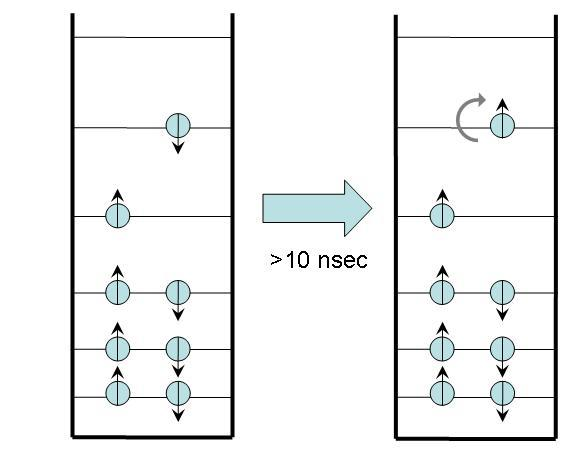
\includegraphics[width=4.0in]{./figures/Topic7/Fig7-4.jpg}
	\caption{Intersystem crossing.}
	\label{Fig7-4}
\end{figure}

The details of the oxygen spin states is beyond the scope of this course. However, a schematic is shown in Fig.~\ref{Fig7-5}, where two singlet states and one triplet state are due to differences in how molecular orbitals are filled to result in varying total spin (red arrows). It is only three four of the 2p electrons responsible for the singlet-triplet states. The singlet state denoted $^1\Sigma_g^+$ is very short lived and converts to the more common singlet state denoted $^1\Delta_g$. This singlet state is reactive due to one oxygen appearing to have a completely filled orbital, while the other appears to have an unpaired electron. This is a higher energy, very reactive state. The triplet state is denoted $^3\Sigma_g^-$.
\begin{figure}[h]
	\centering
	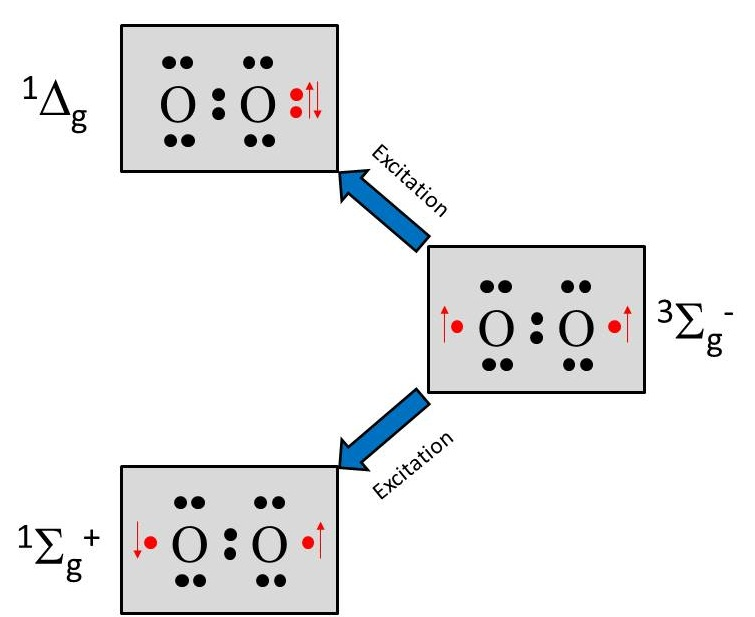
\includegraphics[width=3.5in]{./figures/Topic7/Fig7-5.jpg}
	\caption{Electronic structure of singlet and triplet oxygen.}
	\label{Fig7-5}
\end{figure}

Triplet states have long lifetimes, ranging from a fraction of a millisecond to several seconds.  They last until the electrons encounter a strong electric field disturbance or another high-spin molecule.  For example, a triplet-state organic molecule reacts readily with a triplet-state oxygen molecule (the normal state of this molecule), deactivating both to the singlet state: 
$$^3{\rm molecule}+^3{\rm O}_2 \rightarrow ^1{\rm molecule}+^1{\rm O}_2.$$
Singlet oxygen is a very reactive free radical.  In porphyria, sunlight activates most of the metal-free hemes near the surface of the skin to the triplet state.  When they react with $^3{\rm O}_2$ in the skin, $^1{\rm O}_2$ forms, which further reacts to inflame nearby tissue.  Patients often experience extreme photosensitivity and must avoid sunlight.  For this reason, the disease has been cited as a possible source of werewolf and vampire legends.

Photodynamic therapy (PDT), often used to treat skin cancer, uses the ability of photoexcited molecules to create $^1{\rm O}_2$.  Some molecules, like porphyrins, are absorbed preferentially by cancer tissue.  After applying a topical porphyrin-based substance to the skin and allowing it to absorb, the skin is irradiated with light.  The singlet oxygen produced by the triplet porphyrin then destroys the cancer tissue.  The technique is also used to treat cancers of the eye and throat.

\section{Phosphorescence}

A molecule that undergoes phosphorescence begins in the excited triplet state and emits a photon to return the molecule to ground state.  Actually, transitioning straight from the triplet state to the ground state violates spin angular momentum; in phosphorescence, quantum processes cause the excited triplet state to become slightly “impure,” entering a metastable triplet state.  When this occurs, the molecule can then emit a photon and return to the ground state.  

\begin{figure}[h]
	\centering
	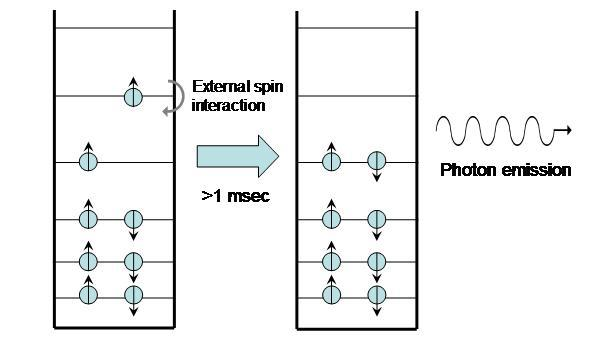
\includegraphics[width=4.0in]{./figures/Topic7/Fig7-6.jpg}
	\caption{Phosphorescence.}
	\label{Fig7-6}
\end{figure}
Because triplet states are so long-lived, the process can take from seconds to minutes.  Glow-in-the-dark watches and other similar products are all based on phosphorescence.

In vivo, phosphorescence is very difficult to observe.  Usually the triplet state is deactivated upon reacting with a ``quencher'' like oxygen before it can phosphoresce from this long-lived state.  If this does not occur, the molecule can undergo energy transfer (Section 7.7) or charge transfer (Section 7.8).  With so many processes to take away the excess energy, we rarely see light emitted through phosphorescence.

\section{Energy Transfer}

Excitation transfer, also called energy transfer, occurs between two molecules: an excited molecule passes its energy to a nearby molecule in its ground state.  The process is illustrated in Fig.~\ref{Fig7-7}. No real photons are ever emitted or exchanged during this process; the electron movement from the excited molecule is ``sensed'' and its energy picked up by the ground-state molecule.  
\begin{figure}[h]
	\centering
	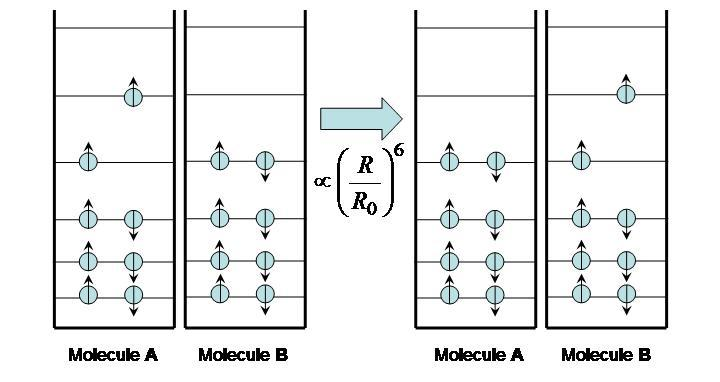
\includegraphics[width=4.5in]{./figures/Topic7/Fig7-7.jpg}
	\caption{Excitation energy transfer between molecules.}
	\label{Fig7-7}
\end{figure}  

The time it takes for excitation transfer to occur is described by F{\"o}rster's relation
$$\tau\propto\left(\frac{R}{R_{\circ}}\right)^6.$$
where $R$ is the distance between molecules and the F{\"o}rster radius $R_{\circ}$ is a constant that depends on the nature of the molecules (roughly ~5 nm).  If $R > R_{\circ}$, the excited molecule A may lose its energy through fluorescence before it can be transferred to B.  If $R < R_{\circ}$, however, energy is efficiently transferred from A to B and fluorescence takes place from the second molecule.  Assuming the fluorescence spectra of the two fluorophores are distinct, it can be determined which case is occurring, as illustrated in Fig.~\ref{Fig7-8}.
\begin{figure}[h]
	\centering
	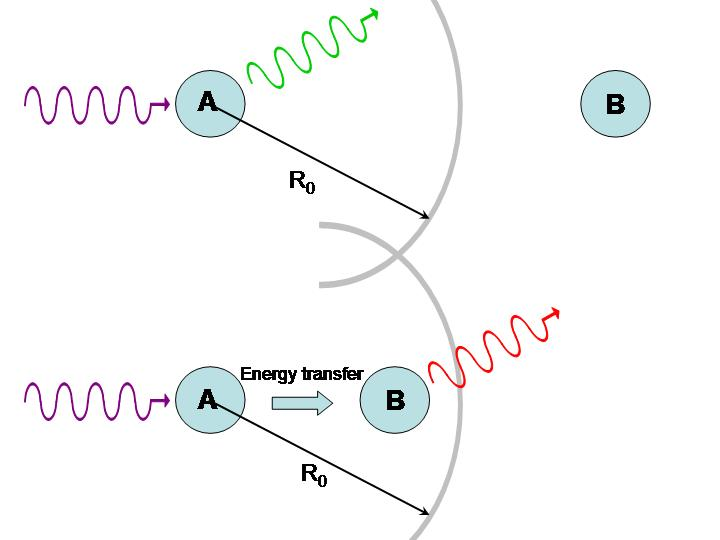
\includegraphics[width=3.75in]{./figures/Topic7/Fig7-8.jpg}
	\caption{Use of energy transfer to infer distances between molecules.}
	\label{Fig7-8}
\end{figure}

If molecules A and B are identical, we cannot tell whether energy transfer is occurring because the energy is continuously swapped between the two.  If they are different, we can illuminate the sample with light of a wavelength absorbed by A but not by B.  If the system is undergoing energy transfer, molecule B will fluoresce light of a different wavelength.  Fluorescence Resonance Energy Transfer (FRET) microscopy exploits this phenomenon to produce images of proteins and other molecules in living cells.  The idea is that when one protein, tagged with a fluorophore A, comes into close proximity of another protein, also tagged with a fluorophore B, energy transfer takes places place from A to B. Thus any site where the emission from B takes place represents a locus for protein-protein interactions. The same technique can be applied to study interactions with DNA and other molecules. 
Excitation transfer is particularly important to photosynthesis.  Chlorophyll molecules normally fluoresce intensely when dissolved in dilute concentrations.  In plants, however, fluorescence is quenched because of energy transfer to other molecules, as depicted in Fig.\ref{Fig7-9}.  Chlorophyll molecules are concentrated in membrane-bound organelles called chloroplasts.  In each of these photosynthetic units, 200-400 chlorophyll molecules are packed around a specialized protein complex called the reaction center.  Collectively, they act like a solar panel.  Once the energy from a photon is absorbed by a chlorophyll molecule, it is transferred to another nearby chlorophyll molecule within a few picoseconds.  The energy is passed back and forth among the so-called “antenna pigments” until it encounters the reaction center.
\begin{figure}[h]
	\centering
	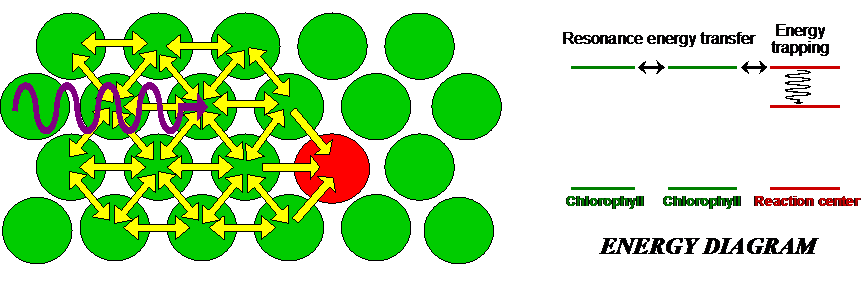
\includegraphics[width=\textwidth]{./figures/Topic7/Fig7-9.png}
	\caption{Antenna pigments are chlorophyll molecules that funnel light to the reaction center of a chloroplast.}
	\label{Fig7-9}
\end{figure}
When the energy from the incoming photons reaches the reaction center, it is trapped and used for chemical reactions.
 
A final example of energy transfer involves the use of $\beta$-carotene to alleviate the harmful effects of photosensitizers, molecules that make something sensitive to light.  When a photosensitizer in the body absorbs light, it undergoes a rapid transition to the triplet state.  In the presence of $\beta$-carotene, the energy from the photosensitizer is transferred to the $\beta$-carotene molecule, which then returns to ground state by undergoing a radiationless transition.  Often taken as an antioxidant, $\beta$-carotene can be found in leafy green vegetables, yellow and orange vegetables, and fruits.  Incidentally, $\beta$-carotene is also used to treat the cutaneous porphyrias.


\section{Charge Transfer}
Like energy transfer, charge transfer occurs between an excited molecule and a ground-state molecule.  However, instead of energy passing between the two, the excited electron is exchanged as depicted in Fig.\ref{Fig7-10}.
\begin{figure}[h]
	\centering
	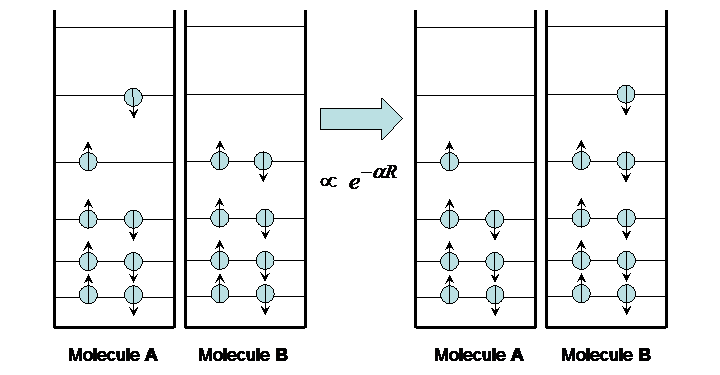
\includegraphics[width=4.5in]{./figures/Topic7/Fig7-10.png}
	\caption{Charge transfer.}
	\label{Fig7-10}
\end{figure}

The transfer occurs on a time scale that varies widely depending on the distance between the two molecules, from picoseconds to seconds.  This time variation is exponential with distance, as expected for the quantum mechanical “tunneling” phenomenon.

\begin{figure}[h]
	\centering
	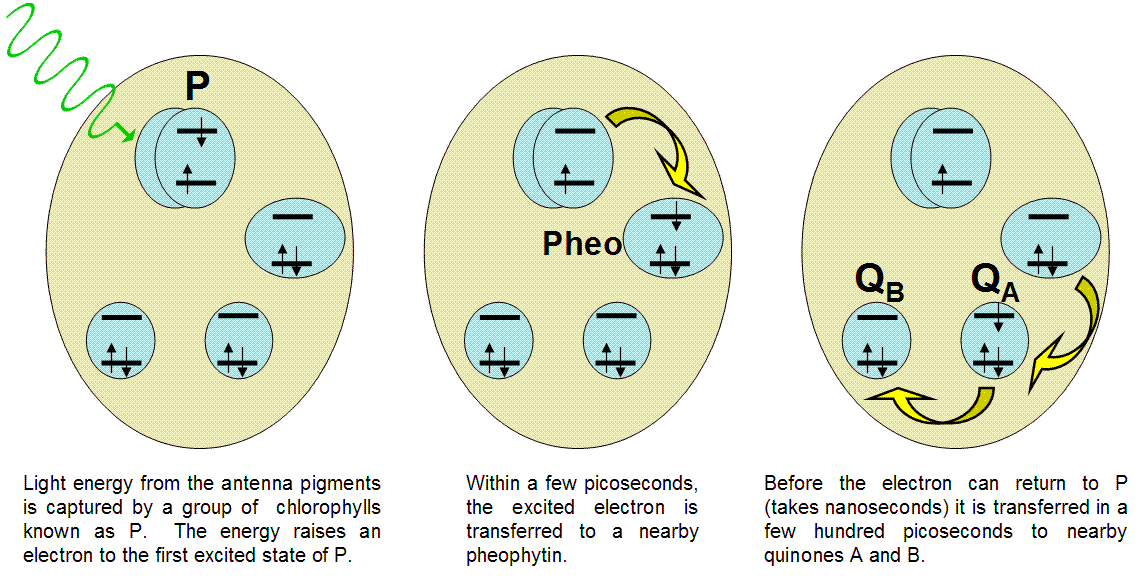
\includegraphics[width=\textwidth]{./figures/Topic7/Fig7-11.png}
	\caption{Events in the reaction center}
	\label{Fig7-11}
\end{figure}
In nature, the best example of light-induced charge transfer is the photosynthetic reaction center.  This protein unit is designed to separate charges faster than they can recombine, providing a source of electrons for chemical reactions.  Fig.\ref{Fig7-10} details the action inside the reaction center.      